\documentclass[10pt,compress,handout]{beamer}
    \useoutertheme{miniframes}
    \usepackage[english]{babel}
    %\usepackage[margin=1in]{geometry}

    \usepackage{amsmath}
    \usepackage{amsfonts} 
    \usepackage{amssymb}
    \usepackage{amsthm}
    \usepackage{mathtools}

    \usepackage[utf8]{inputenc}
    %\usepackage[exscale, amsfonts, amssymb]{concmath}
    %\renewcommand*{\bfseries}{\mdseries}

    \usepackage{float}
    \usepackage{graphicx}
    \usepackage{caption}
    \usepackage{subcaption}

    \graphicspath{{./src/figures/}}

    %\usepackage{fancyhdr} %custom headers and footers layout
    \usepackage{lastpage} %package to print the last page
    %\pagestyle{fancy} %fancy page style

    \usepackage{textcomp} 
    \usepackage{multicol} 
    \usepackage{multirow}

    \usepackage[table]{xcolor}
    \usepackage{booktabs}

    \usepackage[backend=biber,
    bibstyle=ieee, 
    citestyle=numeric-comp,
    natbib=true,
    doi=false, 
    url=false,
    isbn=false,
    mincitenames=1,
    maxcitenames=1,
    minbibnames=1,
    maxbibnames=99,
    backref=false,]
    {biblatex}
    \addbibresource[label=main]{./src/references.bib}

    \usepackage{url}
    \usepackage{hyperref}

    %edit the properties of your PDF documents which will be displayed
    \hypersetup{
        bookmarks=true, 		% show bookmarks bar?
        unicode=true,  		% non-Latin characters in Acrobat’s bookmarks
        pdftoolbar=true,        % show Acrobat’s toolbar?
        pdfmenubar=true,        % show Acrobat’s menu?
        pdffitwindow=true,      % page fit to window when opened
        pdftitle={EIS --- Basics},    % title
        pdfauthor={M. Skocic},     % author
        pdfsubject={},   % subject of the document
        pdfnewwindow=true,      % links in new window
        pdfkeywords={}, % list of keywords
        colorlinks=false,       % false: boxed links; true: colored links
        linkcolor=red,          % color of internal links
        citecolor=green,        % color of links to bibliography
        filecolor=magenta,      % color of file links
        urlcolor=cyan           % color of external links
    }

    \usepackage{tikz}
    \usepackage{circuitikz}
    \usetikzlibrary{decorations.pathmorphing,arrows,calc}

    \title{Electrochemical Impedance Spectroscopy}
    \author{M. Skocic, PhD Electrochemistry and Materials}
    \date{\vfill 
\includegraphics[width=0.70\textwidth]{full_bw.png}}   

    \setlength{\parskip}{6pt}
    \newcommand{\coef}{1}

\begin{document}
    \begin{frame}
        \titlepage
    \end{frame}

    \begin{frame}
        \frametitle{Contents}
        \tableofcontents
    \end{frame}
    
\section{Introduction}
    \begin{frame}{Introduction}
        There are 2 categories of electrochemical techniques: 
        time domain and frequency domain \citep{bard2001}.

        Time domain :
        \begin{itemize}
            \item Voltammetry: $I=f(U)$.
            \item Chronoamperometry: $\Delta U$, $I(t)$.
            \item Zero Resistance Ammeter: $\int j_{gal} \cdot dt$.
            \item \ldots
        \end{itemize}

        Frequency domain:
        \begin{itemize}
            \item Electrochemical Impedance Spectroscopy: EIS.
            \item PhotoElectrochemical Impedance Spectroscopy: PEIS.
        \end{itemize}

        Advantages of EIS:
        \begin{itemize}
            \item Measurement in small perturbations (approximately linear).
            \item Different processes have different time constants.
            \item Large frequency range from $\mu Hz$ to $GHz$.
        \end{itemize}
    \end{frame}

\section{Basics}
    \begin{frame}{Black Box Approach}
        Assume a black box with terminals.

        One applies a voltage and measures the current response (or vice versa).

        Periodic signal with an angular frequency $\omega = 2\pi f$
        with $0 \le \omega < \infty$:
        \begin{itemize}
            \item Voltage $V(\omega) = V_0 e^{j \omega t}$  
            \item Voltage $I(\omega) = I_0 e^{j \omega t - \Phi}$  
        \end{itemize}
        
        \begin{columns}
            \centering
            \column{0.3\textwidth}\centering
                \begin{figure}[h]
                    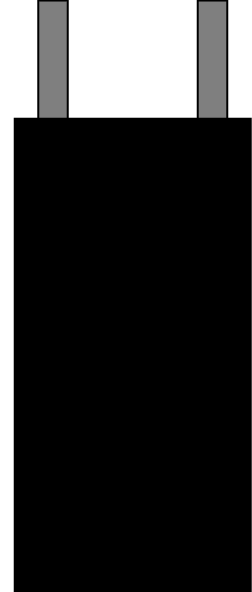
\includegraphics[width=0.5\textwidth]{EIS-black_box}
                \end{figure}
            \column{0.35\textwidth}\centering
                \begin{figure}
                    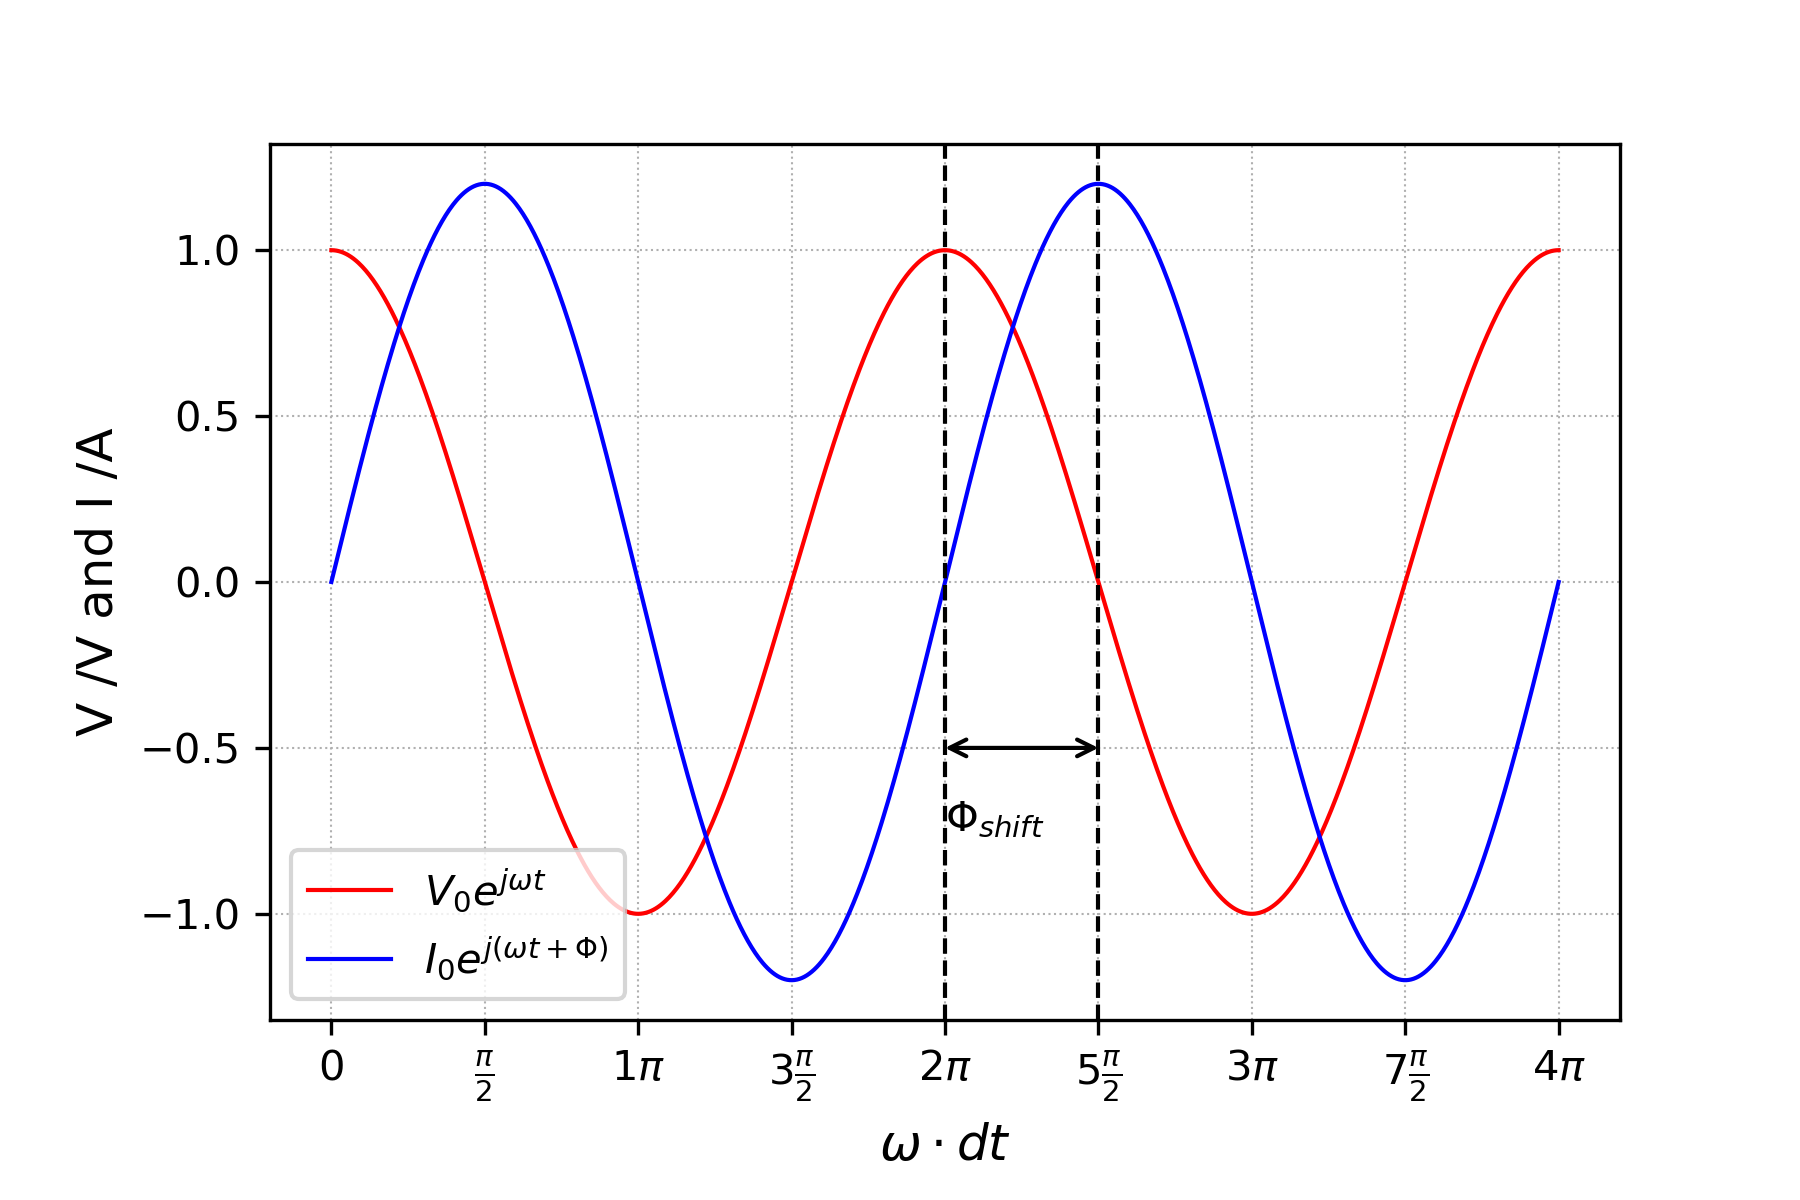
\includegraphics[width=\textwidth]{EIS-ac_waves}
                \end{figure}
            \column{0.35\textwidth}\centering
                \begin{figure}
                    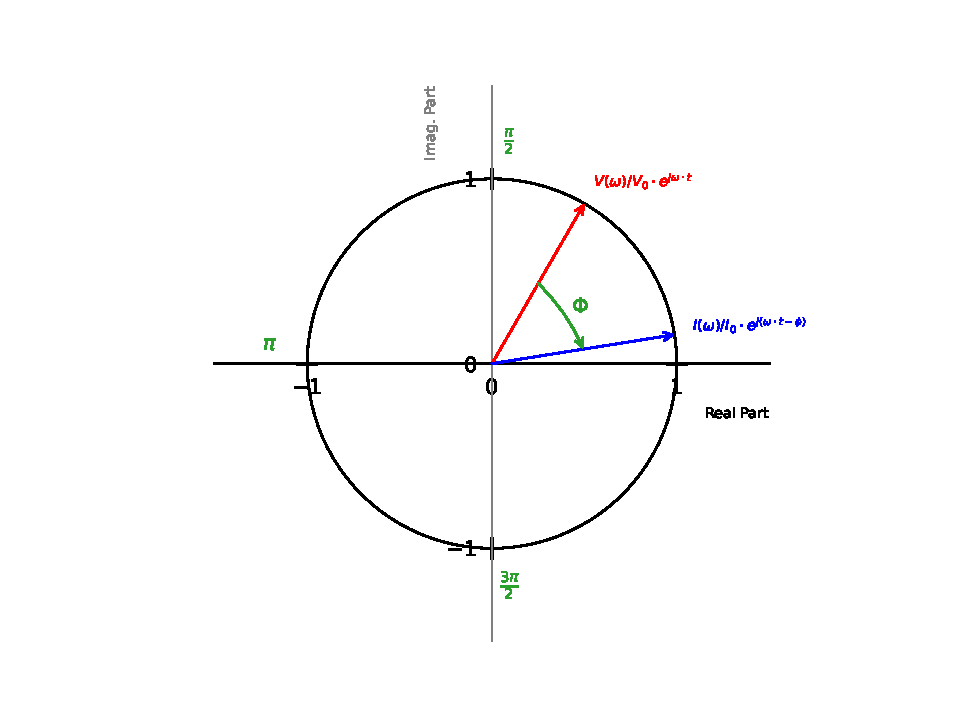
\includegraphics[width=1.3\textwidth]{EIS-ac_waves-trigcircle}
                \end{figure}
        \end{columns}
    \end{frame}
    
    \begin{frame}{What is EIS?}
        The complex impedance is determined from the imposed voltage/current and the measured
        current/voltage through the Ohm's law:
        $$ Z(\omega) = \frac{V(\omega)}{I(\omega)} = \frac{V_0}{I_0} e^{j \Phi} = Z_0 e^{j\Phi}$$

        Therefore:
        \begin{itemize}
            \item  resistive behavior: $ReZ=Z_0 \cdot \cos \Phi$
            \item  capacitive/Inductive behavior $ImZ=Z_0 \cdot \sin \Phi$
        \end{itemize}
        
        Sometimes, the complex admittance $Y(\omega)$ can also be used which is defined as the inverse of the
        complex impedance $Z(\omega)$ 
        $$Y(\omega)=\frac{1}{Z(\omega)}$$
    \end{frame}

    \begin{frame}[allowframebreaks=1.0]{Representations}
        The impedance $Z(\omega)$ can be represented in two different ways:
        \begin{itemize}
            \item  Nyquist plot: represents the real and imaginary parts of $Z(\omega)$ using cartesian coordinates.
            \item  Bode plot: shows the phase shift and magnitude changes in the rang of applied frequencies.
        \end{itemize}
    
        The Bode plot has great advantages for observing phase changes. 
        Therefore, it is useful for the study of sensors, filters, and transistors in electronic devices.
        
        The Nyquist plot provides a better insight into the possible mechanisms.

        \framebreak
        Among these two types of representations, the Nyquist plot is more often used to analyze the characteristics of
        electrochemical processes occurring during corrosion.
        \begin{columns}
            \centering
            \column{0.33\textwidth}
                \centering
                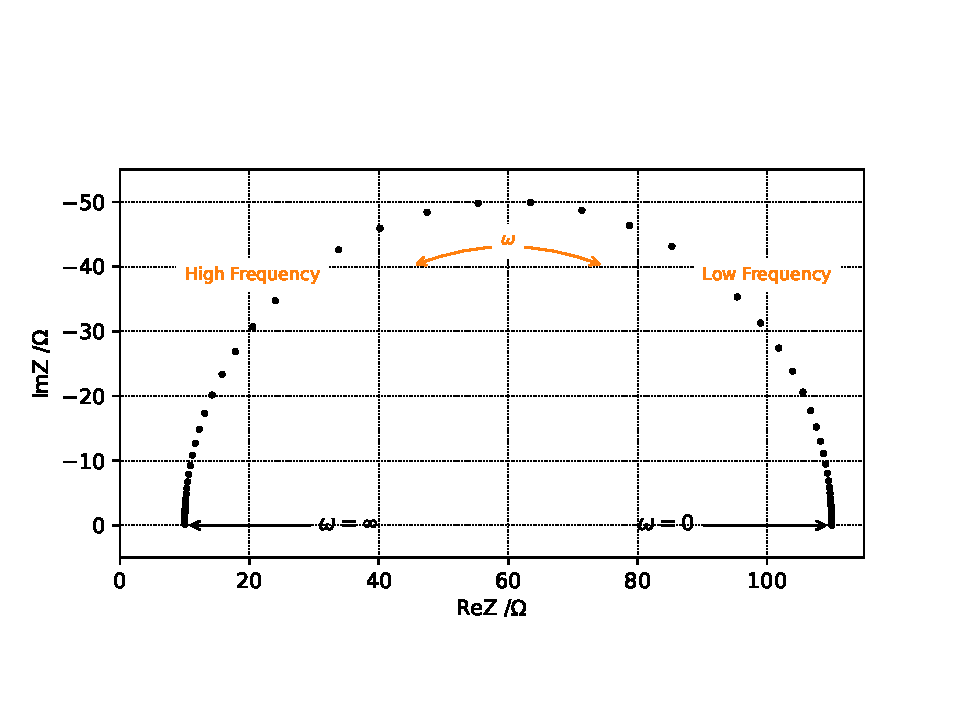
\includegraphics[width=\textwidth]{EIS-example-np}
                Nyquist Plot
            \column{0.33\textwidth}
                \centering
                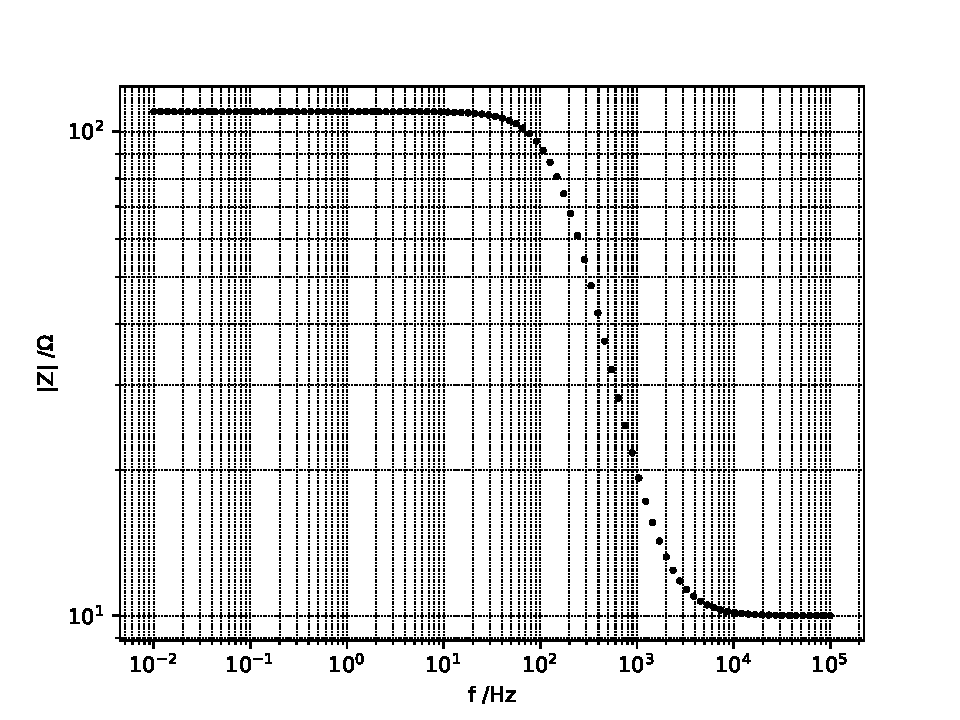
\includegraphics[width=\textwidth]{EIS-example-bm}
                Bode Plot - Modulus
            \column{0.33\textwidth}
                \centering
                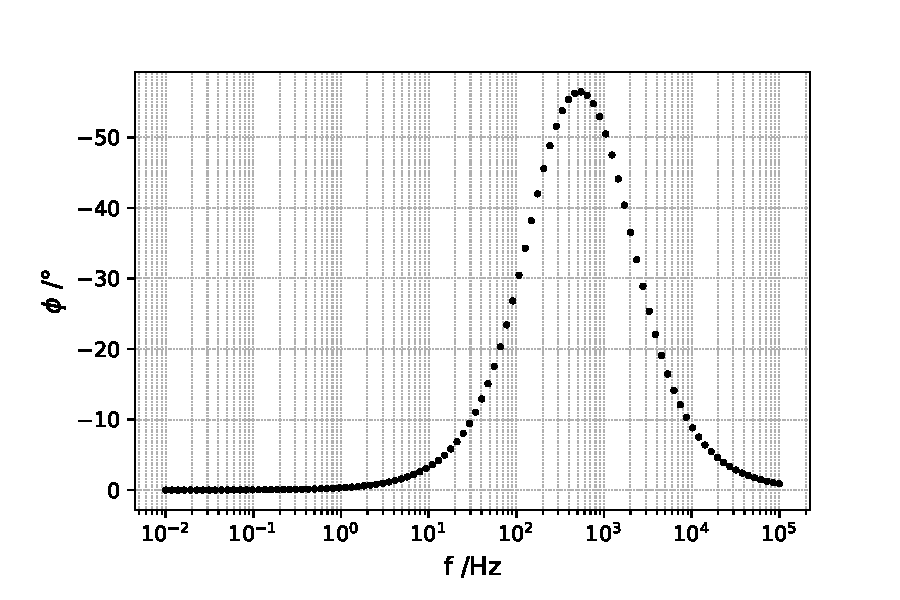
\includegraphics[width=\textwidth]{EIS-example-bp}
                Bode Plot - Phase
        \end{columns}
    \end{frame}

    \begin{frame}{Series and parallel connections}
        Series connections: $Z_1$ --- $Z_2$ --- \ldots --- $Z_n$
        $$ Z_{eq} = \sum _{i=1}^n Z_i $$

        Parallel connections: $Z_1$ / $Z_2$ / \ldots / $Z_n$ 
        $$ \frac{1}{Z_{eq}} = \sum _{i+1}^n \frac{1}{Z_i} $$
        $$ Z_{eq} = \left( \sum _{i=1}^n \frac{1}{Z_i} \right)^{-1} $$
    \end{frame}

    \begin{frame}{Equivalent Circuit Models}
        The circuit model for EIS consists of a combination of electrical circuit elements:
        \begin{itemize}
            \item ideal elements:
            \begin{itemize}
                \item  resistors (R)
                \item  capacitors (C)
                \item inductors (L)
            \end{itemize}
            \item nonideal capacitor-like element: Constant Phase Element (CPE or Q)
            \item diffusion elements:
            \begin{itemize}
                \item semi-infinite Warburg (W)
                \item Finite Length Warburg ($W_{\delta}$ or O)
                \item Finite Space Warburg ($W_m$ or T)
            \end{itemize}
        \end{itemize}
        The circuit model represents the entire system of the electrochemical cell.
    
        The aim is to build an optimal circuit model that is physically meaningful and minimizes the
        number of variables.
    \end{frame}

    \begin{frame}{Circuit Elements}
        
    \end{frame}
    
    \begin{frame}{Circuit Elements and Physical Parameters}
        
    \end{frame}
    
    \begin{frame}{Simplified Randles Circuit}
        
    \end{frame}

    \begin{frame}{Randles Circuit}
        
    \end{frame}

\section{Applications}

% BIBLIOGRAPHY
\begin{frame}[allowframebreaks=0.9]{References}
\AtNextBibliography{\tiny}
%\nocite{*}
\printbibliography
\end{frame}

\end{document}
